\section{L'interface Web}
%\addcontentsline{toc}{section}{L'interface web}

L'interface web est celle qui sera sans doute la plus utilisée car dès que l'on est en établissement scolaire, peu importe les blocages ou les applications, la certitude de trouver un navigateur dans chaque ordinateur est quasi absolue.
\begin{figure}
	\centering
	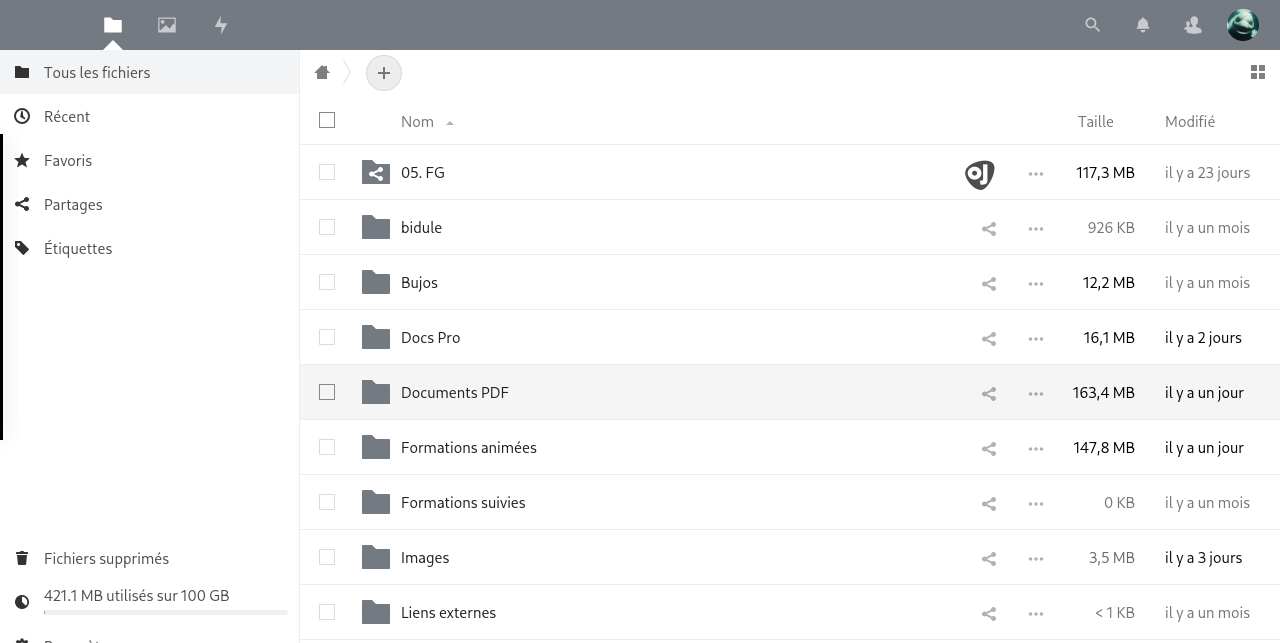
\includegraphics[width=\linewidth]{./Captures/nuage.accueil.png}
	\caption{Le nuage en mode détaillé}
\end{figure}
L'interface est visible en mode mosaïque également.
\begin{figure}
	\centering
	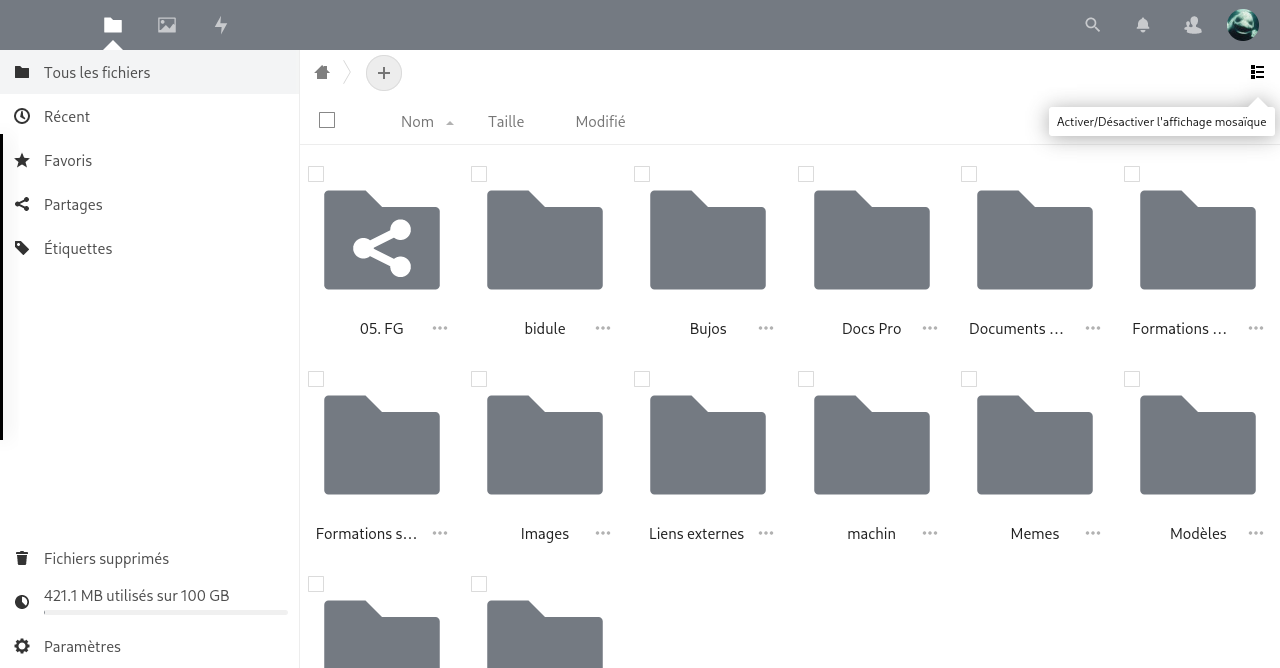
\includegraphics[width=\linewidth]{./Captures/nuage.accueil.mozaique.png}
	\caption{Le nuage en mode mosaïque.}
\end{figure}
L'intérêt de cette interface est de pouvoir y déposer ou récupérer un ou plusieurs fichiers, ou bien un ou plusieurs dossiers. 
L'autre intérêt est que le site étant en ``education.fr'' il ne sera donc pas filtré par les systèmes de pare-feu académiques et évitera l'emploi de clés USB qui se promènent entre le domicile et l'établissement où les niveau de sécurité sont très différents.

